
%% using aastex version 6
\documentclass[twocolumn]{aastex6}

% These are the available options:
%   manuscript	: onecolumn, doublespace, 12pt fonts
%   preprint	: onecolumn, single space, 10pt fonts
%   preprint2	: twocolumn, single space, 10pt fonts
%   twocolumn	: a two column article. Probably not needed, but here just in case.
%   onecolumn	: a one column article; default option.
%   twocolappendix: make 2 column appendix
%   onecolappendix: make 1 column appendix is the default. 
%   astrosymb	: Loads Astrosymb font and define \astrocommands. 
%   tighten	: Makes baselineskip slightly smaller
%   times	: uses times font instead of the default
%   linenumbers	: turn on lineno package.
%   trackchanges : required to see the revision mark up and print output
%   numberedappendix: Labels appendix sections A, B, ... This is the default.
%   appendixfloats: Needed. Resets figure and table counters to zero

\usepackage{verbatim}
\usepackage{amsmath}
\usepackage{graphicx}
\usepackage{cleveref}
\usepackage{hyperref}
\usepackage[normalem]{ulem}

\usepackage{xcolor}

\newcommand{\vdag}{(v)^\dagger}
\newcommand\aastex{AAS\TeX}
\newcommand\latex{La\TeX}
\newcommand{\rr}[1]{$r_{#1}$}
\newcommand{\M}[1]{$M_{#1}$}
\newcommand{\A}{\textit{A}}
\newcommand{\N}{\textit{N}}
\newcommand{\Ps}{$P_{S,0}$}
\newcommand{\Pn}{$P_{N,0}$}
\newcommand{\p}{$p_0$}
\newcommand{\ts}{$t_s$}
\newcommand{\tn}{$t_n$}


%%%%%%%%%%%%%%%%%%%%%%%%%%%%%%%%%%%%%%%%%%%%%%%%%%%%%%%%%%%%%%
%% The following commented section outlines numerous optional output that
%% can be displayed in the front matter or as running meta-data.
%%
%% You can insert a short comment on the title page using the command below.
%% \slugcomment{Not to appear in Nonlearned J., 45.}
%%
%% If you wish, you may supply running head information, although
%% this information may be modified by the editorial offices.
%%\shorttitle{\aastex sample article}
%%\shortauthors{Schwarz et al.}
%%
%% You can add a light gray and diagonal water-mark to the first page 
%% with this command:
%% \watermark{text}
%% where "text", e.g. DRAFT, is the text to appear.  If the text is 
%% long you can control the water-mark size with:
%% \setwatermarkfontsize{dimension}
%% where dimension is any recognized LaTeX dimension, e.g. pt, in, etc.
%%
%%%%%%%%%%%%%%%%%%%%%%%%%%%%%%%%%%%%%%%%%%%%%%%%%%%%%%%%%%%%%%%%%%%


\begin{document}


\title{Galaxy Zoo EXPRESS: Integrating human and machine intelligence in morphology classification tasks}

%% Use \author, \affil, plus the \and command to format author and affiliation 
%% information.  If done correctly the peer review system will be able to
%% automatically put the author and affiliation information from the manuscript
%% and save the corresponding author the trouble of entering it by hand.
%%
%% The \affil should be used to document primary affiliations and the
%% \altaffil should be used for secondary affiliations, titles, or email.

%% Authors with the same affiliation can be grouped in a single
%% \author and \affil call.
\author{Melanie Beck, Claudia Scarlata, Lucy Fortson}%\altaffilmark{1}
\affil{Minnesota Institute for Astrophysics, University of Minnesota, Minneapolis, MN 55454}

\author{Chris Lintott}
\affil{Department of Physics, University of Oxford, Oxford OX1 3RH}

\author{Phil Marshall}

%\altaffiltext{1}{AAS Journals Data Scientist}

%% Mark off the abstract in the ``abstract'' environment. 
\begin{abstract}

We implemented one of the first human-machine combos by running a kick ass
simulation on previous citizen science data in conjunction with machine algorithms. 
And guess what? We can obtain at least an ORDER OF MAGNITUDE improvement in the 
efficiency of classification. So we got that going for us. Which is nice. 

\end{abstract}

%% Keywords should appear after the \end{abstract} command. 
%% See the online documentation for the full list of available subject
%% keywords and the rules for their use.
\keywords{editorials, notices --- 
miscellaneous --- catalogs --- surveys}


\section{Introduction} \label{sec:intro}
The age of Big Data is upon us. Has been upon us. The astrophysics comnunity is 
already shifting focus, preparing for the way in which our science will change and 
the way in which we perform our science will chagne. Look at the new CasJobs -- 
This is the type of shit we need: where analytical tools are integrated at the source
of the data repository. Downloading datasets is a thing of the past. you can't do 
Big Data science if you have to constantly move dem data around. 

Another area we need to get ready for is how we label all that shit in the sky. 
We absolutely love labelling things and it's damn necessary too! And the more sky
we see both in terms of area and depth is going to grow huge AF. We need to find 
efficient, clever ways of picking out transients, radio shits, gravitational lenses, 
galaxy morphology, .... make a really big list with things that are rare or common
or time-domain-y. LSST, Euclid, WFIRST are going to swamp us. 

In this paper we consider the particular problem of galaxy morphology. This 
challenge is actually several combined because it necessitates the need to 
identify the mundane from the unique or rare and, ideally, requires an incredible
amount of detail in order to withdraw useful science. Additionally, morphology is
a great place to start because we can already begin to plan for the future by 
considering the Data of Today. The imaging techniques of future surveys will 
change mostly in resolution and depth; things we can account for. 

Another great reason to use morphology as an example is that we can draw on 
vast, well-established citizen science projects which have contributed to several 
past publications and have lead to serenditious discovery on multiple occasions. 
There is no doubt that to spurn this resource would be a disservice to science!!!!

So then. Morphology it is. And don't think that morphology is just a waste of time
either. While there is certainly always room for improvement in our classification 
system including the fact that our categories were made up 100 years ago and only 
work for the local universe... putting galaxies into categories helps us learn 
about the way dem galaxies be living their lives. 

%%%-------------------------------------------------------
%%% FIGURE:     GZ EXPRESS Schematic
%%%-------------------------------------------------------
\begin{figure*}[ht!]
%\figurenum{1}
\plotone{GZExpress_schematic_v2.jpg}
\caption{Schematic of our hybrid system. Human classifiers are shown images of galaxies via the Galaxy Zoo web interface. These  classifications are recorded and processed according to section XXX. As a result of the processing, those subjects whose probabilties cross the classification thresholds are passed to the machine classifier as a training sample. The trained machine is then applied to the remaining subjects in the database (test sample). Those subjects which the machine classifies with high confidence are removed from the sample and considered fully classified. The rest remain in the database to be seen by human classifiers. \label{fig:schematic}}
\end{figure*}

The idea of combing human and machine classifications IS NOT NEW. That shit's
old AF and a big topic of study in computer science circles; circles we astronomers
have never been invited to but of which we should still be aware. \textbf{Citations
from Chris go here!} So this idea is not novel. What IS novel is one of the first practical
applications and the ability to explore the repercussions of such a system by 
simulating various outcomes on previously collected data. 


In this paper we consider visual classifications from both citizen scientists through
the use of Galaxy Zoo data as well as expert visual classifications from various 
published catalogs as well as visual classifications from within our own team. We 
will combine these with various parameters which originally sought to automatically
classifiy galaxy morphology. parameters like the Gini coefficient, M20, CAS, etc. 
We'll wrap this all up in a neat little package by throwing it all in the 
supervised machine learning algorithm black box which I'll actually explain.
And out will pop some sweet classifications! 

With all that said, start the paper! Section blah will be the components of the method. Section blah will be detail about post-processing visual classifications. Section blah will be about the machine algorithm. Section blah will be testing the method in various circumstances. Section blah will be results. Section blah will be Discussion/Conclusions. 
What sections do we want? 




\section{Overview of the Method?}
Any system combining human and machine classifications will have a set of generic features which we must replicate.

First, a set of humans willing to classify data on request. We will simulate this using a database of classifications from the Galaxy Zoo project which we can draw on at will. These classifications are processed by a Bayesian code first developed for the Space Warps project (SWAP).

Secondly, we need a machine classifier; for this project, we have developed a random forest classifier using easily measured physical parameters such as CAS and Gini as input. See Section X for details.

Thirdly, we will need to make decisions about how the two sets of classifications are combined. After a batch of (human) classifications is processed, then the machine will be trained and its performance assessed against a validation sample. This process is repeated and the machine will grow in accuracy as the size of the training sample increases. Once the machine reaches some acceptable level of performance it is run against the remaining galaxy sample. Images reliably classified by machine are not further classified by humans.

Even with this simple description, one can see that classification will proceed in three phases. At first, the machine will not reach the acceptable level of performance and the only galaxies retired from classified are those for which human classifiers have reached consensus. Secondly, the machine will rapidly improve and both human and machine classifiers will be responsible for image retirement. Finally, improvement in the machine performance will slow, and the remaining images will need to be classified by humans. Working in this allows even moderately successful machine learning routines to be used alongside human classifiers and removes the need for ever-increasing performance in machine classification.


%%----------------------------------------------------------------------------------------------------------------------------------------------------
%%   Galaxy Zoo 2 Data Description
%%----------------------------------------------------------------------------------------------------------------------------------------------------
\section{Galaxy Zoo 2 Classification Data} \label{sec:data}

Our simulations utilize original classifications made by volunteers during the GZ2 project. 
These data are described in detail in \citep{Willett2013} though we provide a brief overview here.  
The GZ2 subject sample was designed to consist of the brightest 25\% ($r$ band magnitude $< 17$) 
of resolved galaxies residing in the SDSS North Galactic Cap region from Data Release 7 
and included both subjects with spectroscopic and photometric redshifts out to $z < 0.25$.
In total, 285,962 subjects were classified in the GZ2 Main Sample catalogs (reference website?). 
Of these, 243,500 have spectroscopic redshifts while 42,462 have only photometric redshifts.  

Subjects were shown as color composite images via a web-based interface wherein 
volunteers answered a series of questions pertaining to the morphology of the subject.
In terms of GZ2, a \textit{classification} is defined as the total amount of information about a subject 
obtained by completing all tasks in the decision tree. A \textit{task} represents a segment of the
tree consisting of a \textit{question} and possible \textit{responses}. 
With the exception of the first task, subsequent tasks were
dependent on volunteer responses from the previous task creating the decision tree 
as shown in Fig~\ref{fig: decisiontree}.
 In total, the data consist of over 14 million classifications from 83,943 individual volunteers. 

%%%-------------------------------------------------------
%%% GZ EDECISION TREE
%%%-------------------------------------------------------
%\begin{figure*}[]
%\figurenum{1}
%\plotone{gz2_decisiontree.pdf}
%\caption{.Galaxy Zoo 2 decision tree. For our first simulation we use only the top level task: ``Is the galaxy simply smooht and rounded, with no sign of a disk?" \label{fig: decisiontree}}
%\end{figure*}


Our first simulated run considers only the first task in the decision tree: 
`Is the galaxy simply smooth and rounded, with no sign of a disk?', to which possible 
responses include `smooth', `feature or disk', and `star or artifact'.  Because all 
volunteers see the first task, our simulations are run with as many as 14,144,941 
classifications.  The SWAP software requires that each classification consist of at least
volunteer ID, subject ID, timestamp of the classification,  and the volunteer's vote.



%%----------------------------------------------------------------------------------------------------------------------------------------------------
%%   Talk About SWAP 
%%----------------------------------------------------------------------------------------------------------------------------------------------------
\section{Post-processing of human classifications}

Galaxy Zoo decision trees require a large 
number of independent classifications for each subject where this value is typically 
set at forty individual volunteer classifications. Once a project reaches completion, 
GZ team scientists down-weight inconsistent and unreliable 
volunteers while the vast majority of volunteers are treated equally with no up-weighted volunteers.
While this process reduces input from malicious users and `bots' from contributing to the consensus, 
it doesn't reward consistent and correct volunteers. Furthermore, waiting until project completion 
doesn't allow for efficient utilization of super-users, those volunteers who are exceptional at 
classification tasks. [Do I need to cite something here?]

Instead, GZ:EXPRESS employs software adapted from the Space Warps Zoonivere project 
\citep{Marshall2016} which searched for and successfully found several gravitational lens 
candidates in the CFHT Lensing Survey (cite XXX).  Dubbed SWAP (Space Warps Analysis Pipeline),  
the software predicted the probability that an image contained a gravitational lens given 
volunteers' classifications as well as their past experience. While full details can be found in 
\cite{Marshall2016}, we briefly outline the method here.  

The software assigns each volunteer an \textit{agent} which interprets that volunteer's 
classifications. Each agent assigns a 2 by 2 confusion matrix to their volunteer which encodes
that volunteer's probability of correctly identifying feature `\A'  given that the subject 
actually exhibits feature \A. The confusion matrix also encodes that volunteer's 
probabiliy of correctly identifying
the absense of feature \A~(denoted as \N) given that the subject does not exhibit 
feature \A. The agent updates these probabilities by estimating them as 

\begin{equation}
P(``X" | X, d) \approx \frac{N_{``X"}}{N_{X}}
\end{equation}
where $N_{``X"}$ is the number of classifications the volunteer labeled as type $X$, 
$N_X$ is the number of subjects the volunteer has see that were actually of type $X$,
and $d$ represents the history of the volunteer (all subjects they have seen). 
The software employs two prescriptions for when the 
agent updates the volunteer's confusion matrix. In \textit{Supervised} mode the 
probabilities are only updated after the volunteer identifes a training subject, 
i.e., one which the scientest knows the correct label \textit{a priori} while the
volunteer does not. In \textit{Supervised and Unsupervised} mode, the agent
updates the probabilities after every subject the volunteer identifies.  

In addition to agent probabilities, each subject begins with a prior probability 
that it exhibits feature \A: $P(A) = p_0$. 
When a volunteer makes a classification $C$, Bayes' Theorem is used to derive how 
the agent should update the subject's prior probability into a posterior: 

\begin{equation}
P(A|C) = \frac{ P(C|A) P(A) }{P(C|A) P(A) + P(C|N) P(N)}
\end{equation}
where this value can then be calculated using the elements of the agent's 
confusion matrix. \cite{Marshall2016} show that perfect volunteers (i.e., those 
with $P(``A"| A) = 1.0$ and $P(``N" | N) = 1.0$ would calculate the posterior
probability of the subject to be $1.0$ which is not surprising (perfect classifiers 
are perfect!). However, they also show that \textit{obtuse} classifiers (those with 
$P(``A" | A) = 0.0$ and $P(``N" | N) = 0.0$ also produce a posterior probability 
of $1.0$; demonstrating that obtuse volunteers are just as helpful as perfect volunteers.

As the project progresses, each subject's prior probability is continually updated 
and is nudged to higher or lower probability depending on volunteer classifications. 
Eventually most subjects cross a classification threshold which define wthether that
subject has been confirmed or rejected for exhibiting feature \A~and the subject
is considered to be retired.  The software no longer records volunteer information 
for these subjects. 

\subsection{Volunteer Training Sample}

Finally, another key feature of the original Space Warps project was the training of 
individual volunteers through the use of simulated lensed galaxies. Volunteers were 
shown simulated images interspersed with actual data with the simulated data shown
predominately at the beginning of the project. After a volunteer submitted their 
classification, the system provided feedback depending depending on their answer. 
In the next section we describe how we egineered the GZ2 data to mimic the Space 
Warps setup as closely as possible.

We found that the SWAP software does not perform well there are no designated 
training images. Furthermore, the software requires that these training images
be introduced at the beginning of the project to allow volunteer confusion matrices
to update sufficiently before intense classification of test images commences. 
To mimic this behavior we select a sample of $\sim$3500 SDSS galaxies which 
overlaps the \cite{NairAbraham2010} catalog. This catalog contains $\sim$14K 
galaxies classified by expert eyes into various TTypes. Thoug helpful, this particular
classification isn't quite apples to apples, as Nair was not being asked the same 
question that GZ2 volunteers were asked.  Instead, we classified this subsample 
amongst the Galaxy Zoo science team by building a small project on the Zooniverse
platform. The question posed to our science team was identical to the original 
question posed to the volunteers. Approximately 15 members of the GZ science team
contributed to these classifications and at least five experts saw each galaxy. Experts 
this case range from advanced graduate students, post docs, and several 
seasoned faculty members. Once
classification was complete, the votes were aggregated and a simple majority was 
used to provide `expert' labels (`Featured` or `Not`) to the 3500 galaxies. 

While 3500 galaxies is a sizeable undertaking for a handful of experts, it is not a
large sample compared to the GZ2 data set. Thus, not every volunteer saw at least 
one of these ad-hoc training images. Because we wish to recreate the conditions 
of the Space Warps project, we remove from our data all volunteers who never 
classify at leaset one of these 3500 galaxies. This reduces our raw data set from
16 million clicks to 14 million; from XXX unique volunteers to 33K. 

We now have a retroactively designated training sample. When considering the 
raw data base, however, the classifications for these particular galaxies could 
have timestamps anywhere within the 14 month time span during which the original project ran.
As previously stated, SWAP does not perform adequately unless the bulk of the
training occurs at the beginning of a project's life. We therefore adjust the order
of the classification timestamps such that annotations of training sample galaxies
have timestamps well before all other GZ2 galaxies. Since it is implicitly assumed
that a galaxy's classifications are independent and random (galaxy images are 
shown randomly to volunteers), the order of the classifications should have only
as small effect, if any, on the results.  When running a simulation, which
pulls from the database according to timestamps, the training images will be the 
first to be processed through SWAP. 

We have done our best to mimic the Space Warps project with the goal of producing 
meaningful results in a similar format. What we cannot reproduce at this time, however,
is actual volunteer feedback. Space Warps gently guided their volunteers towards 
proper classification in real time by providing pop-up comments during the project. 
We obviously cannot reproduce this behavior after the fact though this difference
should be kept in mind. We discuss this topic further is Section XXX Future Shits. 

%%----------------------------------------------------------------------------------------------------------------------------------------------------
%%   Subsection: specifics of SWAP in context of simulations (sans Machine)
%%----------------------------------------------------------------------------------------------------------------------------------------------------
\subsection{SWAP Requirements}

To simulate a live project we run SWAP on a regular timestep which we set as $\Delta t = 1$ day. 
At each timestep, the software pulls from the database all volunteer classifications which
have timestamps within that range. Before the simulation can be run, a number 
of parameters which control the behavior of SWAP must first be chosen. These include
 the initial confusion matrix assigned to each volunteer, the classification
thresholds and the prior probability of the subject. Specifically, we must choose 
\begin{itemize}
\item \Ps, the initial probability that a volunteer identifies a subject as being 'Smooth', $P_0(``S"|S)$
\item \Pn, the initial probability that a volunteer identifies a subject as being 'Not Smooth', $P_0(``N"|N)$
\item $p_0$, the prior probability of a subject to be `Smooth'.
\item \ts, the threshold defining the minimum probability for a subject to be classified `Smooth'
\item \tn, the threshold defining the maximum probability for a subject to be classified `Not Smooth'
\end{itemize}


%%%-------------------------------------------------------
%%%  FIGURE:    SWAP retired_per_day
%%%-------------------------------------------------------
\begin{figure*}[ht!]
\plotone{retired_per_day_sup_PLPD5_p5_standard2_raw_92days.png}
\caption{Simulation of top level GZ2 question reprocessed using the SWAP software only. In shaded grey are the actual number of volunteer votes. The blue shows the cumulative number of retired subjects according to the original GZ2 retirement scheme whereby a subject must achieve forty volunteer votes. The orange and yellow shading represents the cumulative number of retired subjects according to the SWAP retirement system, in that subject probabilities must cross an appropriate threshold for being labeled as having a feature or not. \label{fig:swapresults}}
\end{figure*}

We perform several simulations to explore SWAP performance compared to the
original GZ2 project in terms of overall accuracy achieved and, perhaps more importantly, 
in terms of time efficiency. Thus, to evaluate SWAP performance we consider two basic metrics:
the cumulative sum of classified subjects at a given point in GZ2 project time, $c_{tot}$, and the 
accuracy of those classifications as compared to the GZ2  labels, $c_{acc}$. \citep{Willett2013}
advise caution when using the GZ2 catalog to select subsamples of galaxies with a given
morphology.  They define various thresholds to aid the community in sample selection of
clean or complete samples. In this case, we want to give a label to every object in the catalog. 
Every subject is given three different type of vote fractions: raw, weighted, and debiased. 
GZ2 debiased vote fractions are calculated to correct morphological classifications for the
 effects of redshift bias, a task that SWAP was not built to handle. 
GZ2 weighted vote fractions serve to downgrade malicious volunteers and/or bots, a task
SWAP was intended to perform as well.  However, because the mechanism for
determining malicious volunteers is entirely different between the two schemes, we 
use GZ2 raw vote fractions as the closest apples to apples comparison. 

Specifically, we take the majority raw vote fraction as the label for that galaxy. If the 
majority resided under `star or artifact' or 'feature or disk', it was labeled as `Featured'; 
otherwise it was labeled as `Not'. We note that under this definition, only 512 subjects
had a majority of `star or artifact' and thus comprise an exceedingly small portion of the
overall sample. 

Figure \ref{fig:swapresults} shows SWAP subject retirement as a function of GZ2
project time compared with the original GZ2 retirement scheme. GZ2 retirement was 
defined as a predetermined number of volunteer classifications. Galaxy Zoo projects
typically require an average of 40 volunteer classifications for consensus. The blue
shaded region represents the cumulative number of retired subjects as a function
of GZ2 project time where we use a more lenient retirement definition: 
namely, if on that day of the GZ2 project, a galaxy had at least 30 classifications, 
it was considered retired. 
 In yellow and orange are the cumulative number of subjects retired
via the SWAP software where retirement is defined by a galaxy's probability
crossing a retirement threshold.  It is immediately obvious that by clever and adaptive 
processing of volunteer classifications speed and efficiency of subject retirement
can be dramatically increased. 


In figure \ref{fig:swapeval} we evaluate the SWAP software by considering
its accuracy, recall and precision (red, blue and green respectively) as compared 
to the GZ2 labels defined by raw vote fractions.  This being a Smooth or Not run
instead of a Featured or Not run, I'm not going to talk about the overall shape
because it's going to change. BOO. These curves are, in part, a 
function of the parameters listed above and we now turn to a discussion of 
how these figures change when one or more of the SWAP parameters is adjusted. 


%%%-------------------------------------------------------
%%%    FIGURE:   SWAP evaluation 
%%%-------------------------------------------------------
\begin{figure}[t!]
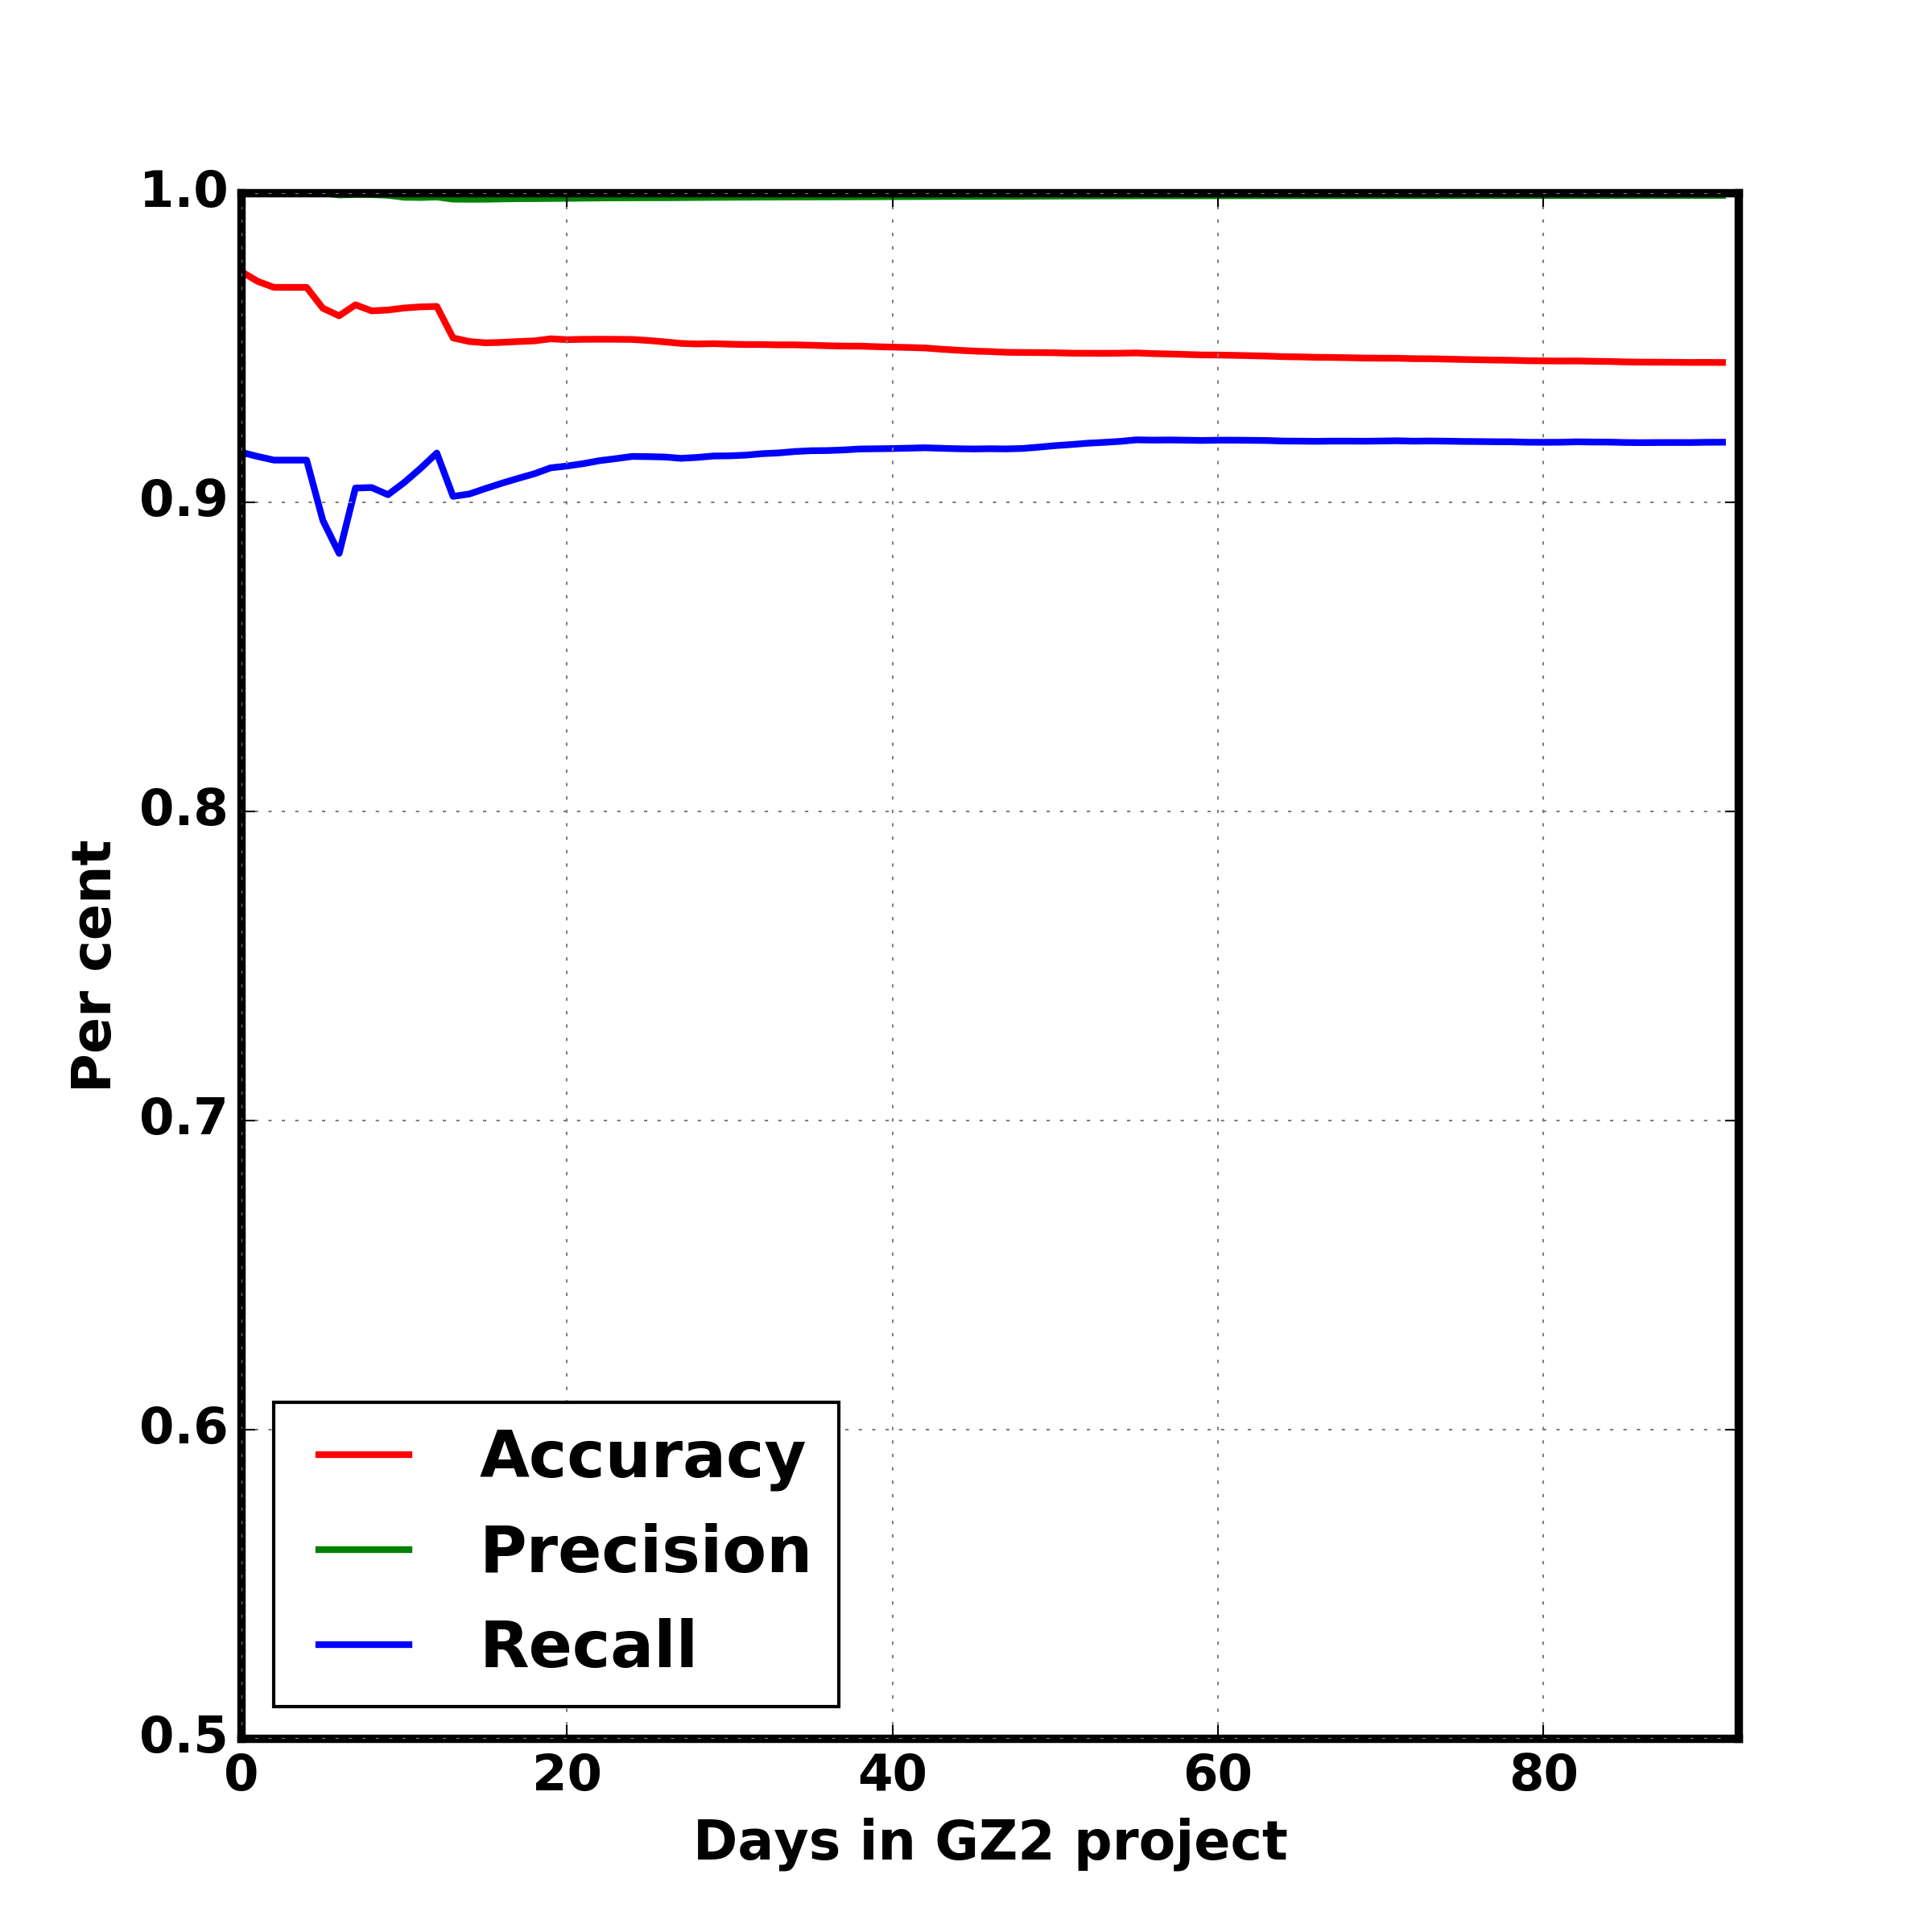
\includegraphics[width=3.5in]{GZX_evaluation_sup_PLPD5_p5_standard2_raw.png}
\caption{GZX evaluation. \label{fig:swapeval}}
\end{figure}

%% ----------------------------------------------------------------------------------------------------------------------------------------------
%% DISCUSSION OF CHANGING SWAP PARAMETERS
%% ----------------------------------------------------------------------------------------------------------------------------------------------
\subsection{SWAP Simulation Outcomes}

\textbf{Initial agent confusion matrix.} 
\begin{figure}[t!]
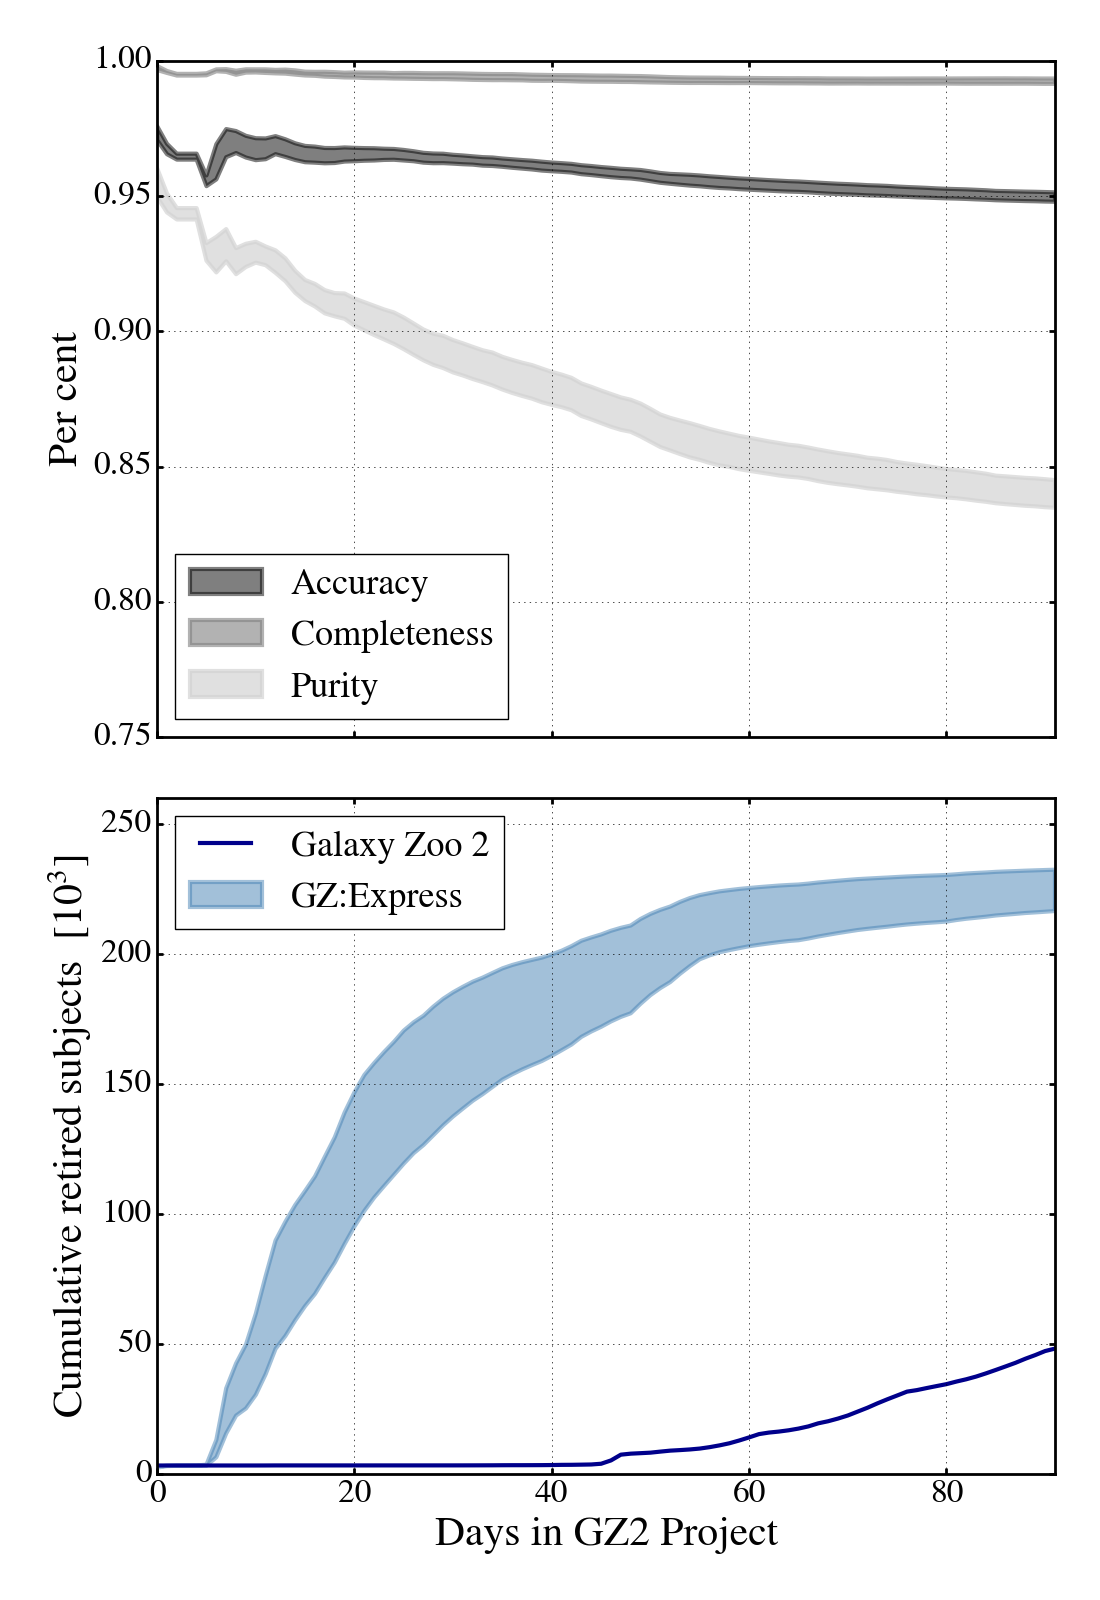
\includegraphics[width=3.5in]{GZX_eval_and_retirement_PLPD_spread_4paper.png}
\caption{GZX/SWAP output as a function of GZ2 project days for a range of initial
confusion matrix values.  \label{fig: confusionMatrixAnalysis}}
\end{figure}
Space Warps agents assigned each volunteer $P(``A"|A), P(``N"|N) = (0.5, 0.5)$, 
assuming that humans started out no better than random classifiers.  We explored a range
of initial confusion matrix probabilities. We find that we are largely insensitive to the 
initial agent confusion matrix values.  The majority of GZ2 volunteers achieve confusion
matrices designating them as astute classifiers, regardless of their initial assigned values. 
The  small variations observed in the SWAP output can be visualized in 
Figure \ref{fig: confusionMatrixAnalysis}. The bottom figure depicts the cumulative 
number of retired subjects as a function of the number of GZ2 project days where the light blue range 
shows the spread due to the initial \Ps~and \Pn~ranging from 0.4 to 0.6. 
Regardless of the initial input values, we achieve a total classification of $\sim225$K  $\pm 3.5\%$ subjects. 
The top figure explores various evaluation metrics as a function of the number of 
GZ2 project days including the overall classification accuracy, completeness, and 
purity of the classification. The spread is within a couple percentage points for any
metric. Overall we maintain accuracy around $95\%$, as well as completeness of $99\%$
while maintaining purity around $84\%$. 


\textbf{Subject prior probability, \p.}
\begin{figure}[t!]
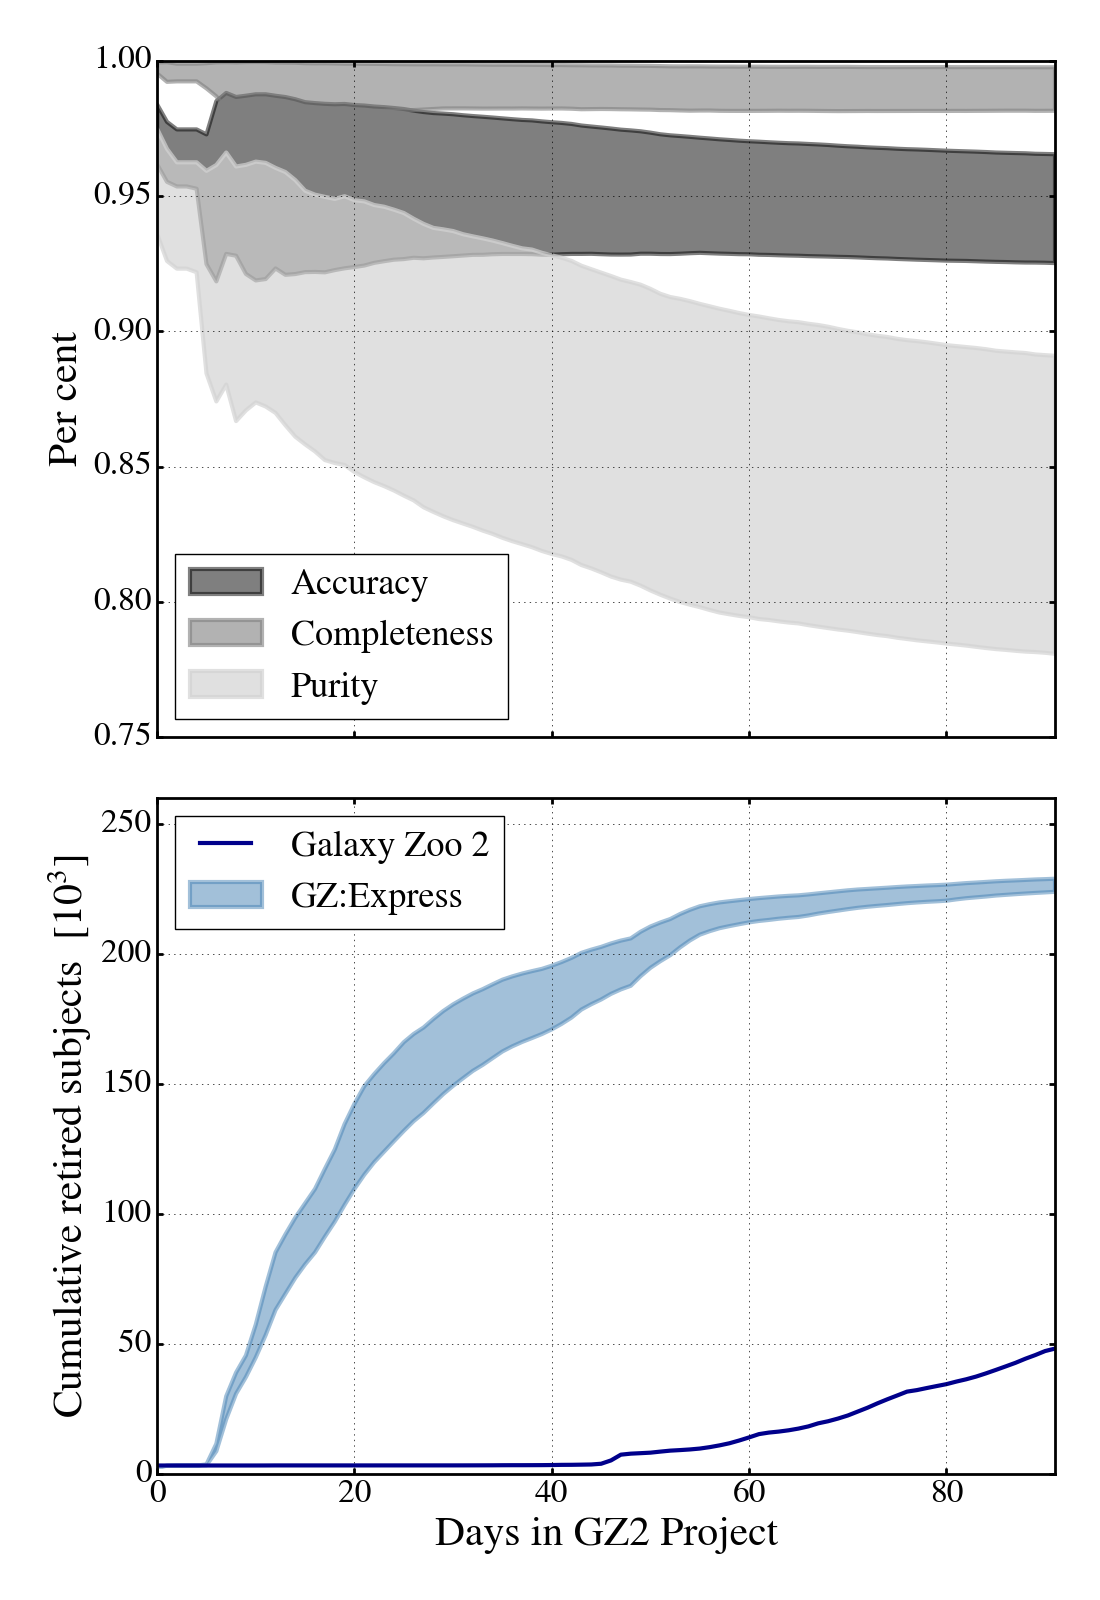
\includegraphics[width=3.5in]{GZX_eval_and_retirement_prior_spread_4paper.png}
\caption{GZX/SWAP output as a function of GZ2 project days for a range of subject prior probabilities.  \label{fig: priorAnalysis}}
\end{figure}
The prior probability assigned to each subject is determined by an educated guess of 
the frequency of that characteristic in the scope of the data at hand. 
For galaxy morphologies, this number should be an estimate of the probability
of observing a desired feature (bar, disk, ring, etc.) within a dataset. In our case, 
we desire to simply find galaxies with any feature at all, however, this is dependent 
on mass and redshift, among other characteristics. The original GZ2 sample was selected
primarily on magnitude, then redshift.  As there was no cut on the galaxy size
(with the exception that each galaxy be larger than the SDSS PSF), the sample
includes a large range of galaxy masses and sizes. As such, designating a single 
prior is not clear-cut. We thus explore how various \p~affect the SWAP outcome.

The bottom panel of figure \ref{fig: priorAnalysis} shows that the overall number
of retired subjects changes very little regardless of \p. In fact, \p~has a smaller effect 
than \Ps~and \Pn~retiring $\sim226$K $\pm1\%$ of subjects over the course of the 
simulated project time. Instead, \p~can change what label a subject is given which, 
in turn, has an effect on evaluation metrics. More subjects are classified as `Not' 
when \p~is small since their prior is already closer to the rejection threshold; 
these same subjects are classifed as `Featured' when \p~is larger.
This explains the larger spread of the evaluation metrics in the top panel of figure 
\ref{fig: priorAnalysis}.  Overall, the average values of accuracy, completeness, 
and purity remain similar over the course of the project compared to figure 
\ref{fig: confusionMatrixAnalysis}. Instead, the spread can 
be as large as $5\%$, in the case of purity. If the desired science is highly contingent
on a pure sample, it falls to the user to choose a prior wisely in order to maximize 
this output. 

How should one go about this task? We find that the prior is, in essence, a reflection
of the dataset at hand. The raw GZ2 classification data are skewed towards labeling 
subjects as `Not', rather than `Featured'. Overall, only 35\% of volunteer votes for 
any subject are \textbf{not} `Smooth'. Knowing this \textit{a priori}, we can set the 
value of \p~$= 0.35$. Everything else remaining constant, we find that this does, 
indeed, maximize SWAP output. 

Thus one could develop a prescription for determining the best \p~for a given dataset
by initializing batches of subjects with various (though intelligently chosen) \p~to 
discover, in real time, which value precisely maximizes output and performance. 


\textbf{Retirement thresholds.}
The Space Warps project set their retirement thresholds equidistant in logspace. 
Their prior was significantly small to begin with as lenses are expected to be very rare.
However, `Smooth' galaxies (which roughly correspond with early-types) are nearly 
equal to the `Not Smooth' within a factor of 2 at low redshift. Thus care must be taken when 
setting \ts~and \tn~for retirement. The SWAP output is most sensitive to these
parameters as they are directly responsible for the label assigned to a given subject. 
When these thresholds are low, subjects more easiliy attain the appropriate 
probability to cross that threshold. This can increase speed of classification however
it also greatly affects accuracy. If the next volunteer disagreed with the previous 
volunteer on the nature of the subject, her vote could bring the probability of
the subject below the threshold and thus it wouldn't yet be classified. 
Therefore setting these values is crucial. 

{\color{red} TO DO: 3. I haven't don't any real analysis of changing thresholds. So get on it!!!}

Summary of this section? Segue into Machine Classifier. Regardless of the parameters
with which one begins (within reason) the number of retired subjects grows significantly. 
GZ2 required at least 48 days before it could retire ~50K subjects whereas SWAP
can retire that many within 4 days, depending on parameter choice / with some 
\% difference? / something like that. It is instructive to consider the number of
volunteer `clicks` instead of the physical timescale as this is a quanity that 
spans multiple projects regardless of the number of volunteers that project may
have. In this light, GZ2 requires nearly $2.5\times10^6$ votes to retire 60K
subjects while, to match it, SWAP requires only $4\times10^5$, an ORDER OF MAGNITUDE REDUCTION BITCHES! 



%%----------------------------------------------------------------------------------------------------------------------------------------------------
%%   INTEGRATING MACHINE CLASSIFIERS 
%%----------------------------------------------------------------------------------------------------------------------------------------------------
\section{Machine Classifier} \label{sec:machine}

Supervised learning is the machine learning task of inference from labeled 
training data. The training data consist of a set of training examples, including
an input (feature) vector and a desired output (or label).  Generally speaking,
a supervised learning algorithm analyzes the training data and produces an inferred 
function that can then be mapped to new examples. An optimized algorithm will 
correctly determine class labels for unseen data. In general, most classification 
algorithms can handle prediction of several labels simultaneously. Work has been
done to predict the entirety of GZ2 classification labels using deep learning 
\citep{Dieleman2015} with great success. However, it is still simpler for a machine
to predict fewer labels than it is to predict several dozen. \textbf{[citation?]} 
Fortunately, by handling individual features and processing human classifications
through SWAP, we arrive with a discrete, binary task for a machine to tackle.
However, in the future we plan to explore more sophisticated algorithms which 
are optimized to handle a continuum since the actual output of the SWAP software
is a probability for any given subject to exhibit a particular feature. 

\subsection{Random Forests}
Because our task is simple, we choose a simple machine. In particular, we use 
a Random Forest (RF) algorithm,  an ensemble classifier that operates by bootstrapping
the training data and constructing a multitude of individual decision tree algorithms, 
one for each subsample.  An individual decision tree works by deciding which of 
the input features best separates the classes. It does this by only performing 
splits on the values of the input feature that most decrease the classification 
error. These feature splits proceed recursively, always with the goal of decreasing 
the classification error. As such, decision trees alone are prone to overfitting the 
training data which precludes them from generalizing well to new data. 
Random Forests mitigate this effect by combining the output label from the 
multitude of decision trees.  In particular we use the 
\texttt{RandomForestClassifier} from the Python module \texttt{scikit-learn}
\citep{scikit-learn}. 

\begin{comment}
\subsubsection{K-nearest neighbors}
%One of the simplest algorithms to conceptualize and use is the K-nearest neighbors (KNN) classifier. This classifier works simply by considering the K neighbors nearest to the test point in Euclidean space. As we have only a binary classification challenge, the test point is classified according to the majority of its K neighbors. In the event of a tie, the label if the closest neighbor to the test point determines its class. Though simplistic, this algorithm is surprisingly powerful in that it performs well in higher-dimensional space and is relatively fast to train. Obviously, the most important parameter to consider is the number of nearest neighbors to assign to each test point. But this is pretty much the only knob to turn in this method which is another benefit -- ease of interpretation. 
%We use scikit-learn's implementation of K-Nearest Neighbor Classifier (KNC) and optimize the K parameter. 
\end{comment}


\subsection{Cross-validation}
Of fundamental importance is the task of choosing an algorithm's hyperparameters, 
values which determine how the machine learns.  In the case of a RF, one must 
choose the maximum depth of the tree, the minimum leaf size, the maximum
number of leaf nodes, etc. The goal is to determine which values will optimize 
the machine's performance and thus cannot be choosen \textit{a priori}. 
Idealy, one would train the machine with every combination of parameters and 
consider the resulting performance by testing the trained machine on a sample
withheld from the training sample so as not to contaminate the results. 
Formally, we perform k-fold cross-validation whereby the training sample is split
into $k$ subsamples. One such subsample is withheld while the remaining data is
used to train the machine. This is performed $k$ times and the average performance
value is recorded. The entire process is repeated for every combination of the 
specified hyperparameter space and the optimal values can be recovered. 

 
\subsection{Feature Representation and Pre-Processing}
Machine learning algorithms require a feature vector for each training example. 
This vector is composed of D individual numeric quantities associated with the 
subject which the machine will use to discern that subject from others in the 
training sample. To segregate `Smooth` from `Not Smooth` our feature set draws 
on ZEST \citep{Scarlata2007} and  is composed of Concentration, Asymmetry, Gini, 
M20 and ellipticity (See Appendix \ref{sec:Appendix} for details concerning the 
measurement process). Altogether, these features describe a five dimensional 
parameter space in which the machine attempts to distinguish the two classes. 
The RF algorithm is capabale of handling a considerable number of features and in
a future paper we will explore increasing this feature space to include parameters
like Sersic index, B/T ratio, color, etc. 
%Good examples include various color metrics, Sersic index, and B/T ratio, among others. 

%\textbf{Should this paragraph be here? Probably not. But it should be somewhere?}
%This is quite distinct from \textit{deep learning} methods which can learn on every 
%pixel of an image through a series of non-linear transformations. This technique has
%been successful at predicting galaxy morphology labels as explored by 
%\cite{Huertas-Company2015}, \cite{Dieleman2015} and others. In this work our focus
%is to outline a practical method to efficiently combine human and machine classification,
%not seek the most optimal or accurate machine algorithm. We are concerned more 
%with speed and simplicity though we stress that a machine is just an algorithm. 
%In the future, this particular application will accommodate any algorithm, including 
%deep learning techniques, should they so be desired. 

%Though deep learning methods promise new heights of classification accuracy, there are some drawbacks. Most notably, the interpration of these methods in the context of physical quantities is lacking. Because of the complex suite of layered non-linear transformations, it is difficult to backstrapolate what qualities of the image were most successful at understanding that galaxy's morphology. Moreover, connecting that to physical mechanisms within the galaxy remains to be seen. On the other hand, much work has been invested in connecting aggregate features such as CAS, G-M20 which are well demonstrated to correlate with specific galaxy stuffs like SFH and ... whatnots.. and described below.

\textbf{THIS STEP NO LONGER NEEDS TO BE DONE -- RF SHOULDN'T CARE:}

{\color{red} TO DO: 4. Check that I'm right! }
Before we feed the algorithm with these feature vectors we first perform two pre-processing steps. First, we clean the data as there are some very few number of cases where our algorithm failed to recover appropriate values for the Petrosian radius, C, A, G, or M20. Our code represents these failures as infs or nans and we thus remove these subjects from all samples.  The second transformation puts each of the features on equal footing. Taken at face value, each of the five morphology parameters resides in a different range of values:  M20 is nearly always negative as it is logarithmic, while Asymmetry and Gini are always between 0 and 1.  In order for the machine classifier to treat all features equally we scale each feature along columns. If a row represents an individual subject, then a column represents the same feature for all subjects. We normalize each subject's features in the standard way: 
\begin{equation}
z_{feature} = \frac{f_i - \mu}{\sigma}
\end{equation} 
Where $f_i$ is the $i$th subject's feature value, $\mu$ is the mean of the entire feature sample, and $\sigma$ is the standard deviation of the entire feature sample. This scales each feature to values between 0 and 1. 


\subsection{Training and Validation Samples}
We are now ready to discuss the training sample. As we showed in the previous 
section, the SWAP software retires subjects much more quickly than the GZ2 project
by adaptively tracking volunteer skill and subject probabilities. This provides us
with a way of quickly generating considerably large subject samples with accurate
labels provided by human classifications. These retired subjets are the basis of the 
machine's training sample. That training sample is dynamically generated as a function
of project time. Within the first week of a project there are perhaps only a few 
subjects which reach retirement, but as the project progresses, that number 
soon becomes thousands.  

As discussed above, in addition to a training sample we also need a validation 
sample to estimate the generalization (true) error of our trained machine. For 
this purpose we maximize the utility of our expertly classified sample. This sample
thus provides training to our volunteers and verification for our machine. 

\subsection{MachineShop Simulation}

As before, we simulate a live project by running our machine directly after
running SWAP and in timesteps of $\Delta t = 1$ day. 
As the simulation progresses each night, a flag associated with each subject is 
triggered in the SWAP software if it reaches retirement. This then signals the 
machine software that it indeed has some amount of training data to consider. 
For our first run, any subject retired by SWAP is immediately considered part of
the machine's training sample, however we do not allow the machine to begin 
learning until it has reached a minimum number of training subjects. For our first
run this number is set to 10K. Once SWAP has reached that number of retired subjects
the machine begins learning. 

The machine is allowed to learn at each timestep. Thus, the machine classifier will 
have some some number, N, of training galaxies. K-fold cross-validation is performed
at each time step to determine optimal hyperparameters. The machine is then trained 
with the optimal parameters and is applied to the validation sample. 
A slew of performance metrics are recorded including the validation accuracy, 
completeness, and contamination. This process repeats at each time step until 
the machine has learned all it can. This requires some discussion.  While it is
true that increasing the sample size will, in general, increase the optimal performance 
of the machine, this behavior eventually reaches a plateau. In order to judge our 
machine as being `fully learned`, we  implement a learning criterion, which 
considers the growing history of the machine's learning and judges the machine
learned after its accuracy varies by less than 1\% over the course of 3 consecutive
timesteps. We will discuss how varying this criterion changes the outcome of the 
classification results. 

Once the machine has been fully trained, it is then applied to the test sample. 
In this case, the test sample is any subject which has either not reached retirement
through the SWAP processing, or is not part of the validation sample. Since the 
total number of subjects in GZ2 is XXX, the validation sample comprises XXX, 
the initial training sample is 10K, thus the first test sample contains XXX subjects. 
The test sample decreases as a function of project time in tandem with the increasing
training sample. Thus the further into the project one goes, the more trained the 
machine becomes and the easier time it has predicting the test sample since that
sample shrinks. 

\subsection{Machine Output}
Once the machine is happily applying itself to the test sample at each timestep, 
we first simply record its predictions along with the probability associated to that
prediction.  Nearly every machine classification algorithm can output a confidence
score or decision function associated with its prediction. In the case of a RF, 
this is calculated as \textbf{[Look this shit up.]} 

In figure \ref{fig:testmetrics},
we can see how the machine is performing on the test sample as a function of 
project time. Understandably, the performance is poor the first time the machine 
crosses the `learnned` criterion. Flukes can happen and it was most likely not
quite as learned as expected or desired. However, as the project progresses the 
performance on the test sample increases. In particular, the black line denotes 
the performance as obtained on the entire test sample and we can see that even 
when the machine is at its peak, the accuracy doesn't increase much beyond 70\%. 
The red line, however, is when we select only those subjects which the machine is
most confident about (more than 90\% confidence, in particular). Now the accuracy
of the machine on this subsample reaches nearly 85\%.  

This allows us to set a criterion for which subjects the machine should be allowed
to retire from the system. We don't necessarily trust it on all subjects but can we 
trust it when it's most confident? Explore this more? 

\subsection{Feedback Loop}
Our system has now incorporated both clever use of human classifications and 
integrated machine classification. We now simulate the final element which is the
feedback mechanism. Those subjects which the machine is most confident about are 
flagged as retired and votes on these subjects are no longer recorded in SWAP or 
elseware. Those which the machine is not confident, however, remain in the pool 
such that, during the next timestep, volunteers can contribute to the classification 
of that subject. This will increase the diversity of the training sample thus 
providing the machine with a larger sample space in which to learn. 

We now perform full simulations, culminating all steps in the method and examine 
the overall performance. 

{\color{red} TO DO: Implement and run this. OY! That's a tall order...}

\section{Results}
Results of a FULL RUN -- including the feedback loop. 


\subsection{Performance \#s}
How well does the overall human/machine system perform together and separately. 

what are sensible criteria for using the machine? If we change these criteria, how does performance change? 

When does the machine kick in? How quickly does it learn? 

Efficency of classification increased by order of magnitude. 


\subsection{The effect of human training}

this all relies on training humans in addition to training machines. 

Fewer users trained

Fewer training images

Less front-loading (how far apart can the training images be staggered and still produce good results?)

This is all qualitative (not fitting functions to anything)

\section{So fucking what?}
All you did was classify Smooth and Not Smooth. Anyone and their mom can do that!


We've now identified several ways to suss out those subjects which require 
additional intervention. If SWAP can't classify it, then potentially these subjects 
should be diverted to experts. If a machine can't classify it, then those subjects
can be relegated back to humans. Thus we have a cute little chain of command!

Apply all these performance metrics to the datasets expected from Euclid, LSST, etc. Estimate reduction in classification time. 








\appendix

\section{Measuring Morphological Parameters on SDSS Cutouts}
\label{sec:Appendix}

So we did a LOT of work to measure all that shit. 


Concetration measures the ... 
\begin{equation}
C = 5\log(r_{80}/ r_{20})
\end{equation}
where \rr{80} and \rr{20} are the radii containing 80\% and 20\% of the galaxy light respectively.  Large values of this ratio tend to indicate disky galaxies, while smaller values correlate with early-type ellipticals. 

Asymmetry quantifies the degree of rotational symmetry in the galaxy light distribution (not necessarily the physical shape of the galaxy as this parameter is not highly sensitive to low surface brightness features).  
\begin{equation}
A = \frac{\sum_{x,y} |I - I_{180}|}{ 2\sum|I|} - B_{180}
\end{equation}
where $I$ is the galaxy flux in each pixel $(x, y)$, $I_{180}$ is the image rotated by 180 degrees about the galaxy's central pixel, and $B_{180}$ is the average asymmetry of the background. 

The Gini coefficient, $G$, describes how uniformly distributed a galaxy's flux is.  If $G$ is 0, the flux is distrubuted homogeneously among all galaxy pixels.; while if $G$ is 1,  all of the light is contained within a single pixel. This term correlates with $C$, however, unlike concentration, $G$ does not require that the flux be concentrated within the central region of the galaxy.  We calculate $G$ by first ordering the pixels by increasing flux value, and then computing
\begin{equation}
G = \frac{1}{|\bar X|n(n-1)}\sum_i^n(2i-n-1)|X_i|
\end{equation}
where $n$ is the number of pixels assigned to the galaxy, and $\bar X$ is the mean pixel value. 

\M{20} is the second order moment of the brightest 20\% of the galaxy flux. 
\begin{eqnarray}
 M_{tot} & = & \sum_i^nf_i[(x_i-x_c)^2 + (y_i-y_c)^2]  \\
 M_{20} & = & \log_{10} (\frac{\sum_iM_i}{M_{tot}}), ~~\textrm{while} \sum_ifi < 0.2f_{tot}
\end{eqnarray}



%% The reference list follows the main body and any appendices.
%% Use LaTeX's thebibliography environment to mark up your reference list.
%% Note \begin{thebibliography} is followed by an empty set of
%% curly braces.  If you forget this, LaTeX will generate the error
%% "Perhaps a missing \item?".
%%
%% thebibliography produces citations in the text using \bibitem-\cite
%% cross-referencing. Each reference is preceded by a
%% \bibitem command that defines in curly braces the KEY that corresponds
%% to the KEY in the \cite commands (see the first section above).
%% Make sure that you provide a unique KEY for every \bibitem or else the
%% paper will not LaTeX. The square brackets should contain
%% the citation text that LaTeX will insert in
%% place of the \cite commands.

%% We have used macros to produce journal name abbreviations.
%% \aastex provides a number of these for the more frequently-cited journals.
%% See the Author Guide for a list of them.

%% Note that the style of the \bibitem labels (in []) is slightly
%% different from previous examples.  The natbib system solves a host
%% of citation expression problems, but it is necessary to clearly
%% delimit the year from the author name used in the citation.
%% See the natbib documentation for more details and options.


\bibliographystyle{apj}
\bibliography{apj-jour,human-machine}

%% This command is needed to show the entire author+affilation list when
%% the collaboration and author truncation commands are used.  It has to
%% go at the end of the manuscript.
%\allauthors

%% Include this line if you are using the \added, \replaced, \deleted
%% commands to see a summary list of all changes at the end of the article.
\listofchanges

\end{document}

%% End of file `sample.tex'.
